% <<<<<< Rapport projet de troisième année >>>>>>

\documentclass[a4paper,12pt,titlepage]{report}
\usepackage[utf8]{inputenc}
\usepackage[T1]{fontenc}
\usepackage{lmodern}
\usepackage[a4paper]{geometry}
\usepackage[french]{babel}
\usepackage{amsmath}
\usepackage{amssymb}
\usepackage{mathrsfs}
\usepackage{hyperref}
\usepackage{graphicx}
\usepackage{appendix}
\usepackage{hyperref}
\usepackage{subcaption}
\usepackage{setspace}
\usepackage[intoc]{nomencl}
%\usepackage{algorithm}
%\usepackage{listing}
\usepackage{verbatim}
\usepackage{fontawesome}

\begin{document}


%==================================== Page de Garde ==============================
\begin{titlepage}
 
	\begin{center}
	\begin{figure}[!h]
	\centering	
		\begin{subfigure}[b]{0.3\textwidth}
		\includegraphics[height = 2cm, keepaspectratio]{graphes/mines_nancy.png}
		\end{subfigure}
		\begin{subfigure}[b]{0.3\textwidth}
		\includegraphics[height = 2cm, keepaspectratio]{graphes/elie_cartan.png}
		\end{subfigure}
		\begin{subfigure}[b]{0.3\textwidth}
		\includegraphics[height = 2cm, keepaspectratio]{graphes/univ_lorraine.png}
	\end{subfigure}
	\end{figure}
 
	\textsc{École nationale supérieure des Mines de Nancy}\\[2cm]
	\textsc{Rapport de projet 3A}\\[1cm]
	\textsc{Pierre Gauthier}\\[1cm]
 
	\begin{doublespace}
		{ \huge \bfseries{Algorithme d'apprentissage en chimie quantique et application au screening (sélection) de cellules photovoltaïques}}\\[2cm]
	\end{doublespace}
	\textmd{Laboratoire : Institut Élie Cartan}\\[1cm]
	\textmd{Tuteurs : Jérémie Unterberg, Marianne Clausel, Dario Rocca}
	% Bottom of the page
	\vfill
	{\textit{{\large 21 Novembre 2018}}}
 
	\end{center}
\end{titlepage}

%================= Table des matières ===============================
\tableofcontents

\newpage



%======================== Introduction ==============================
\textbf{\Huge Introduction:} \\
\newline

Ce projet est conduit dans un cadre pédagogique en tant que projet de troisième année à l'école des Mines de Nancy avec pour tuteurs Marianne Clausel, Dario Rocca et Jérémie Unterberg. Il suit la publication scientifique de Mathias Rupp \textit{Machine Learning for Quantum Mechanics in a Nutshell}.  
Le but du projet est la reproduction des résultats de cette étude, pour ensuite pouvoir proposer des variations dans le traitement et étudier l'influence sur le résultat à travers les différents indicateurs que nous définirons. \\
Les codes sont en annexe, mais sont aussi disponible sur le dépôt Github suivant :  \url{https://github.com/pierrzacharias/Projet_3A}.

%%%%%%%%%%%%%%%%%%%%%%%%%%%%%%%%%%%%%%%%%%%%%%%%%%%%%%%%%%%%%%%%%%%%%
\chapter{Contexte de l'étude}
\section{The Harvard Clean Energie Project}
\paragraph{}
La publication de Mathias Rupp \textit{Machine Learning for Quantum Mechanics in a Nutshell} s'inscrit dans la dynamique des différents travaux menés autour d'un vaste projet de recherche : \textit{The Harvard Clean Energie Project}. Ce projet vise à concevoir une nouvelle gamme de panneaux solaires révolutionnaire conçus à partir de molécules organiques. Ces panneaux permettrait de s'affranchir des terres rares indispensable actuellement, et d'atteindre de meilleur rendement énergétique (15\% selon une source, et d'être beaucoup plus économique que les panneaux actuels par la facilité de production).\\
Toute la problématique du projet est de trouver de nouvelle molécules présentant des propriété optimale pour une utilisation sur des panneaux solaire. 
Les équipes de Harvard sont donc à la recherche de la molécule présentant les caractéristiques optimales parmi un set de l'ordre de 3.5 millions de molécules.
\paragraph{}
Cependant calculer les propriétés des molécules amène à résoudre le problème à N corps, c'est à dire le système d'équation de Schrödinger qui ne comporte pas de solutions analytique. 
Le développement de la théorie de la DFT (\textit{density functional theory}) dans les années 80 pallie à cette difficulté, et permet de calculer les états d'énergie des molécule à partir de l'état fondamental. 
\paragraph{}
Mais le temps de calcul pour étudier toute les molécules reste considérable au vu de leur grand nombre. Le \textit{Clean Energie Project} a notamment en 2011 fait appel à un réseaux de crowd computing : ce sont des réseaux de bénévoles mettant à disposition une partie de la puissance de calcul de leur ordinateur pour des projets à grande échelle du monde scientifique nécessitant un temps de calcul hors du communs.  
\paragraph{}
L'article que cherchons à reproduire explore de nouvelles techniques novatrices de couplage entre la physique quantique et la prédiction de données pour s'affranchir des limitations de puissance de calculs et explorer le maximum de configuration par extrapolation des résultats. \\
\paragraph{}
Nous allons ainsi nous appuyer sur un set de molécules dont les énergies on étés calculé par la théorie de la DFT, et faire de la prédiction pour de nouvelle molécules à partir de ces dernière en employant les méthode de machine learning.

\newpage
\section{Descripteurs des molécules}

\paragraph{}
Nous allons à présent nous intéresser aux données sur lesquelles nous allons effectuer nos prédictions, et quels descripteurs nous allons employer.

\paragraph{}
Initialement, nos données sont les coordonnées de chaque atomes de la molécule, et  l'énergie d'atomisation de celle-ci. \\
Nos données sont alors contenues dans un fichier au format .xyz.
Chaque élément du fichier correspondant à une molécule est un tableau avec en première ligne le nombre d'atome de la molécule, en deuxième ligne l'énergie d'atomisation et le numéro de la molécule dans le fichier, et pour chaque ligne ensuite correspond aux coordonnées cartésienne de l'atome dans la molécule. A noter que ces coordonnées sont par rapport à un atome de référence.\\
\\
\begin{tabular}{ l c c c }
   Nombre d'atome &  & & \quad\\
   numéro de la molécule &\quad énergie d'atomisation &\quad &\\
   atome 1 & x(1) & y(1) & \quad z(1) \\
   atome 2 & x(2) & y(2) & \quad z(2) \\
   . & . & . & \quad . \\
   . & . & . & \quad . \\
   . & . & . & \quad . \\
   atome n & x(n) & y(n) &\quad  z(n) \\
 \end{tabular}
 \\
 \\
 \\
 Par exemple pour la première  molécule du fichier CH$_4$ que l'on traite :
\begin{figure}[!h]
\begin{tabular}{ l c c c c c c}
   5 &  & & \quad\\
   0001 &\quad -417.031 & & & & & \\
   C & 1.04168000 & -0.05620000 & -0.07148000 & 1.04168200 & -0.05620000 & -0.07148100\\
   H  & 2.15109000 & -0.05620000 & -0.07150000 & 2.13089400 & -0.05620200 & -0.07149600\\
   H  & 0.67187000 & 0.17923000 & -1.09059000  &  0.67859800 &  0.17494100 & -1.07204400\\
   H & 0.67188000 & 0.70866000 & 0.64196000 & 0.67861300 &  0.69474600  & 0.62898000\\
   H & 0.67188000 & -1.05649000 & 0.23421000 & 0.67861400 & -1.03828500  &0.22864100\\
 \end{tabular}
 \caption{Premier élément du fichier .xyz correspondant à la première molécule. Le bloc de coordonnées à gauche correspond aux coordonnées du champ de force et le bloc de droite correspond aux coordonnées DFT.}
 \end{figure}
 
\paragraph{}
Nous allons ensuite mettre en forme ces données avec un descripteur pour effectuer nos prédictions par la suite. Nous utilisons les matrices de Coulomb pour représenter les molécules.
Les matrices de Coulomb sont définies comme suit : 
\[
M_{ij} = 
	\left\{
	\begin{array}{ccc}		
	\begin{aligned}
		& 0.5 Z_{i}^{2.4} \quad &i=j\\
		& \frac{Z_i Z_j}{||R_i - R_j||_{2}} \quad &i\neq j
	\end{aligned}
\end{array}
	\right.
\]
avec $Z_i$ le numéro atomique correspondant et $R_i$ la position des atomes.\\


\paragraph{}
Dans la pratique, les calculs que nous allons mettre en place pour la prédiction nécessite un nombre constant de descripteur par molécules, même si celle-ci n'ont pas le même nombre d'atomes et donc des matrice de Coulomb de taille variante.
Nous allons donc remplir pour chaque molécule une matrice de Coulomb de taille égale au nombre maximal d'atome que nous pouvons avoir parmi les molécules que l'on considère ans notre jeu de données, c'est à dire un matrice de taille 23$times$23.

\paragraph{}
Les matrices de Coulomb sont symétriques ce qui fait que nous pouvons garder que la partie inférieure ou supérieure de la matrice pour la prédiction. Nous allons ainsi conserver la partir supérieure de la matrice de Coulomb dans un vecteur de taille $\frac{23\times(23+1)}{2} = 276$.

\paragraph{}
On veillera dans ce procédé à conserver les termes nuls de la matrice initiale de taille $23\times23$ pour que les descripteurs identiques puissent être également positionnée dans le vecteur final. On peut voir l'importance de cette remarque sur  un court exemple sur deux molécules : CH et CH$_2$ :
\paragraph{}
Pour C-H :
\begin{tabular}{ l | c c c c }
	 & C 	& H 	&   &		\\
	 \hline
   C & a$_1$ & b$_1$ &  0 & 0   \\
   H & b$_1$ & a$_2$ &	0 & 0	\\
    & 0 & 0 & 0 & 0	 \\
   & 0 & 0 & 0 & 0 \\
    \end{tabular} \\
Ce qui donne le vecteur ( a$_1$, b$_1$, 0, 0, a$_2$, 0, 0, 0, 0, 0) \\
Pour H-C-H on retrouve les même termes :
\begin{tabular}{ l | c c c c }
	 & C 	& H 	&   &		\\
	 \hline
   C & a$_1$ & b$_1$ &  c$_1$ & 0   \\
   H & b$_1$ & a$_2$ &	c$_2$ & 0	\\
   H & c$_1$ & c$_2$ &	a$_3$ & 0	\\
   & 0 & 0 & 0 & 0 \\
    \end{tabular} \\
 Ce qui donne le vecteur ( a$_1$, b$_1$, c$_1$, 0, b$_1$, a$_2$, c$_2$,0 ,a$_3$, 0, 0)
 \paragraph{}
On voit dans cet exemple l'importance de conserver les termes nuls lors du remplissage du vecteur, pour que les termes égaux correspondant à des atomes dans des situations semblables soient positionnée à la même place, notamment les termes diagonaux qui ne dépendent que de l'atome lui-même. Sinon les modèle que nous mettrons en place pour la prédiction seront faussés.

\paragraph{}
De plus comme nous l'avons énoncé,les coordonnées des atomes sont déterminées par rapport à un atome de référence ce qui fait que les matrices de coulomb ne sont pas insensibles aux inversions de ligne pour les modèle de régression. Pour que toute les matrices soient équivalents de ce point de vue la, nous trions les lignes de la matrice par norme descendante, en inversant les lignes correspondante pour conserver la symétrie de la matrice avant de prendre la partie diagonale supérieure.\\

\paragraph{}
Sur le Github \url{https://github.com/pierrzacharias/Projet_3A} la mise en 
forme des données telle que décrite dans cette section se trouve dans le 
fichier de code \textit{ecriture{$\_$}Matrice{$\_$}de{$\_$}Coulomb.py} dans le dossier \\
\textit{Ecriture{$\_$}des{$\_$}Matrices{$\_$}de{$\_$}Coulomb/}. Elle sont encodés en sortie 
dans le fichier \textit{matrice{$\_$}coulomb.txt}
%%%%%%%%%%%%%%%%%%%%%%%% Chapitre 1 %%%%%%%%%%%%%%%%%%%%%%%%%%%
\chapter{Modèle de prédiction : Machine learning}
\label{C1}
%%%%%%%%%%%%%%%%%%%%%%%%% sectioon 1 %%%%%%%%%%%%%%%%%%%%%%%%%%%%%%
\section{Support Vector Machines methods (SVM)}
\paragraph{}
Nous considérons les données : $(x_{i},\ y_{i})_{1 \leqslant i \leqslant N},\ x_{i} \in \mathbb{R}, \ y_{i} \in \{-1,\ 1\}$.
\paragraph{}
Le probléme SVM vise à séparer les données  en deux classes $+1$ et $-1$ à l'aide de la fonction $f(x) = w \cdot x + b \ (b \in \mathbb{R},\ w \in  \mathbb{R}^{d})$ telle que :
\[ \begin{aligned}
	f(x) > 0 &\Rightarrow x \in C_{+1} \\
	f(x) < 0 &\Rightarrow x \in C_{-1} 
	\end{aligned}
\]

\begin{figure}[!h]
	\begin{center}
	\centering	
	%\begin{subfigure}[b]{0.3\textwidth}
		\includegraphics[height = 5cm, keepaspectratio]{graphes/SVM_donnee.png}
		\includegraphics[height = 5cm, keepaspectratio]{graphes/SVM_separee.png}
		\caption{sparation de données générées make$\_$blobs du package dataset et séparation de l'espace en deux classe par la méthode des vecteurs support à l'aide de la fonction SVC du package sklearn. Les étoiles sont les vecteurs supports.}
			%\end{subfigure}
	\end{center}
\end{figure}
Nous voulons trouver l'hyperplan qui sépare le mieux nos données parmi tous ceux compatibles.

\paragraph{}
Pour juger la qualité d’un hyperplan en tant que séparateur on utilise la distance entre les données et l'hyperplan. Plus précisément, la « marge » d’un problème d'apprentissage est définie comme la distance entre l’hyperplan de séparation et l'individu le plus proche . \\
Pour un hyperplan $H$ = $\{x$ | $w^T x + b =0\}$, on a :
\[
\text{Marge}(H) = \text{min}_{x_{i}}\ d(x_i,\ H)
\]
\begin{figure}[!h]
	\begin{center}
	\centering	
	%\begin{subfigure}[b]{0.3\textwidth}
		\includegraphics[height =5cm, keepaspectratio]{graphes/svm05.png}
		\caption{Illustratin de la distance à l'Hyperplan H.[Cours Cnam RCP209] }
			%\end{subfigure}
	\end{center}
\end{figure}
\begin{figure}[!h]
	\begin{center}
	\centering	
	%\begin{subfigure}[b]{0.3\textwidth}
		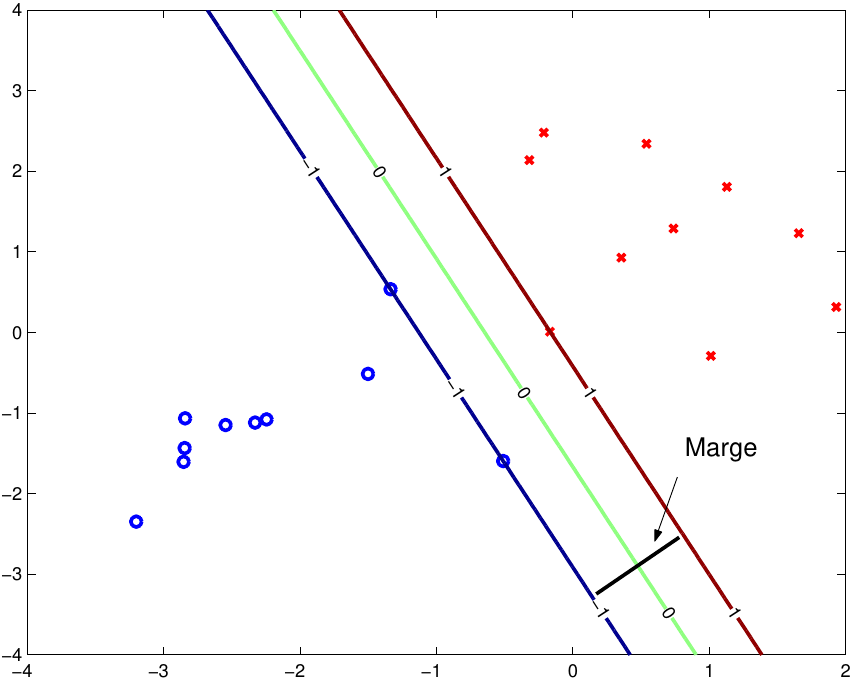
\includegraphics[height =5cm, keepaspectratio]{graphes/svm04.png}
		\caption{Le meilleur hyperplan parmi tous ceux compatible est, comme on le voit ici, celui qui passe au \og millieu \fg des données, et donc celui qui maximise la marge. C’est le séparateur de marge maximale.[Cours Cnam RCP209]}
			%\end{subfigure}
	\end{center}
\end{figure}
\paragraph{}
On définit alors les vecteurs supports comme les éléments les plus proches de part et d'autre de l'hyperplan de séparation qui déterminent la marge (Figure 2.4)
\begin{figure}[!h]
	\begin{center}
	\centering	
	%\begin{subfigure}[b]{0.3\textwidth}
		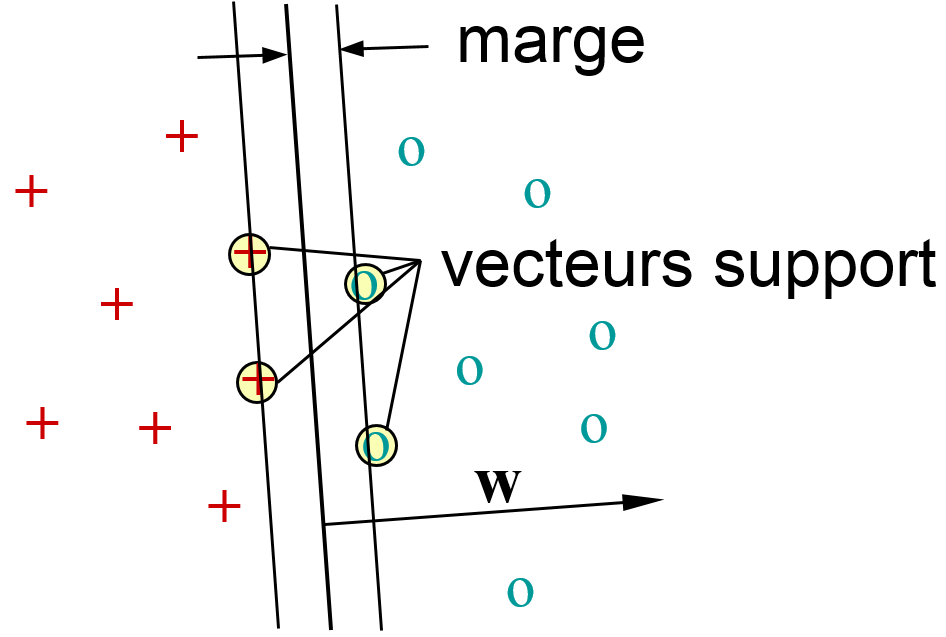
\includegraphics[height =5cm, keepaspectratio]{graphes/svm07.png}
		\caption{Le meilleur hyperplan parmi tous ceux compatible est, comme on le voit ici, celui qui passe au \og millieu \fg des données, et donc celui qui maximise la marge. C’est le séparateur de marge maximale.[Cours Cnam RCP209]}
			%\end{subfigure}
	\end{center}
\end{figure}
\paragraph{}
On peut ainsi exprimer la marge en fonction des vecteurs supports $x_{vs}$:
\[ 
2 \times \text{Marge} = 2 \times d(x,\ H) = \frac{|w^T x_{vs} + b|}{||w||}
\]
Nous prendrons dans la suite la quantité 2$\times$ Marge car cela ne change pas le problème de minimisation et simplifie les expressions. On impose pour les vecteur supports $|w^T x_{vs} + b| = 1$. La marge devient donc :
\[ \text{Marge} = \frac{2}{||w||} \]

Sous l'hypothèse qu'il existe un hyperplan qui sépare nos données, trouver l'hyperplan qui maximise la marge revient à résoudre le problème suivant:
\[
	\left\{
	\begin{array}{ccc}		
	\begin{aligned}
		&\text{arg}\ \text{min}_{w,b}\ \frac{1}{2}||w||^{2} \\
		&\forall \ 1 \leqslant i \leqslant N,\ y_i (w \cdot x_i + b)\geqslant 1
	\end{aligned}
\end{array}
	\right.
% − \sum{ \lambda_{i} (y_{i} (w \cdot x_i + b)−1)}
\]

On utilise le Lagrangien des conditions de Karush, Kuhn et Tucker, qui s'exprime sous la forme suivante :
\[
L(w,b,\lambda_{i}) = \frac{1}{2}||w||^{2} - \sum{\lambda_{i}( y_i (w \cdot x_i + b)-1)}
\]
Le problème de minimisation trouve sa solution pour les paramètres ($w$, $b$, $\lambda$ tels que: 
\[
\left\{
	\begin{array}{cc}		
	\begin{aligned}
		\frac{\partial L}{\partial b}(w^*, b^* , \lambda^*) &= 0\\
		\frac{\partial L}{\partial w}(w^*, b^* , \lambda^*) &= 0
	\end{aligned}
\end{array}
	\right.
\]
Ce qui amène à :
\[
\left\{
	\begin{array}{cc}		
	\begin{aligned}
		\sum_{i=1}^{n}{\lambda^{*}_i y_i} &= 0\\
		\sum_{i=1}^{n}{\lambda^{*}_i y_i x_i} &= w^*
	\end{aligned}
\end{array}
	\right.
\]
Ce qui permet d'obtenir l'expression du problème dual :
\[
\left\{
\begin{array}{lll}
	\text{max}\ L(\lambda) = \sum_{i}{\lambda_{i}} - \frac{1}{2} \sum_{i}{\sum_{j}	{\lambda_{i} \lambda_{j} y_i y_j x_i \cdot x_j}} \\
 \lambda_i \geqslant 0 \\
 \sum_{i}\lambda_i y_i = 0 
\end{array}
\right.
\]
avec le paramètre $b^*$ que nous obtenons avec la relation $|x_{vs}^T w^*  + b^*| = 1$ que nous avons fixée précédemment.
La fonction de décision correspondant à la solution du problème de maximisation de la marge est :
\[
	f^* (x) = \sum_{i=1}^n {\lambda^*_i y_i x^T_i x + b^*}
\]

%%%%%%%%%%%%%%%%%%%%%%%%%%%%%%%%%%%%%%%%%%%%%%%%%%%%%%%%%%%%%%%%%%%%%%%%%%%%%%%
\section{Données non-linéairement séparables : Astuce du noyaux.}
%%%%%%%%%%%%%%%%%%%%%%%%%%%%%%%%%%%%%%%%%%%%%%%%%%%%%%%%%%%%%%%%%%%%%%%%%%%%%%%%
\paragraph{}
Dans la section précédente nous avons considéré des données linéairement séparable,
nous allons à présent nous intéresser au cas où il n'existe pas d'hyperplan qui puissent séparer nos données. L'idée principale de cette section pour pouvoir séparer nos données et de passer dans un base de dimension supérieure telle que nos données deviennent linéairement séparables comme cela est illustré sur la figure 2.5.

\paragraph{}
Pour ce faire nous allons remplacer le produit scalaire $x^T x$ dans l'expression de $f$ par une fonction dite \og noyaux \fg : $K : \xi \times \xi \rightarrow \mathbb{R}$. \\
On donne quelques exemple de noyaux courant en figure 2.6. Logiquement, comme nous cherchons à séparer les données, les noyaux prennent des valeurs importante pour des données proches.

\begin{figure}[!h]
	\begin{center}
	%\begin{subfigure}[b]{0.3\textwidth}
		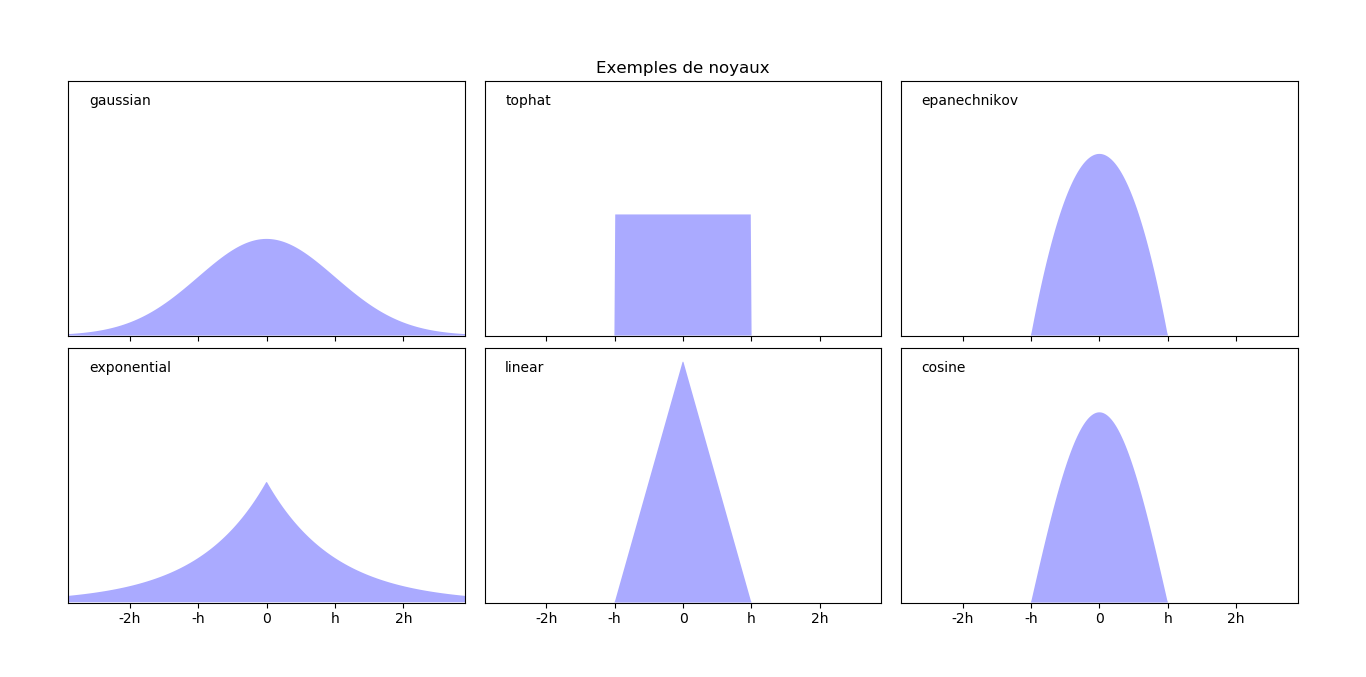
\includegraphics[height = 5cm, keepaspectratio]{graphes/exemple_noyaux.png}
		\caption{Affichage de la densité pour des noyaux courant [Documentation scikit-learn]}
			%\end{subfigure}
	\end{center}
\end{figure}

\paragraph{}
Les fonctions noyaux $K$ doivent vérifier les conditions de Mercer :
\begin{itemize}
\item[$\bullet$]  $K$ est continue symétrique 
\item[$\bullet$]  $K(x_i,x_j)_{\ 1 \leqslant i,j \leqslant N}$ est une matrice définie positive
\end{itemize}
\paragraph{}
Le théorème de Mercer nous assure ainsi de l'existence d'un espace de Hilbert $H$ et d'une fonction $\phi :\xi \rightarrow H$ telle que $K(x,y) = \langle\phi(x),\phi(y)\rangle$.

\begin{figure}[!h]
	\begin{center}
	%\begin{subfigure}[b]{0.3\textwidth}
		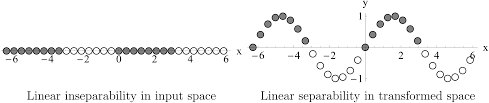
\includegraphics[height = 3cm, keepaspectratio]{graphes/separation.png}
		\caption{Astuce du noyaux : projeter les données dans un espace de dimension plus grande, où elles deviennent séparables linéairement.[Mathias Rupp\textit{Machine Learning for Quantum Mechanics in a Nutshell}]}
			%\end{subfigure}
	\end{center}
\end{figure}

L'estimateur devient ainsi en effectuant le produit scalaire sur l'ensemble des données $(x_{i})_{1 \leqslant i \leqslant N}$:
\[
f(\overset{\sim}{x}) = \sum_{i = 1}^{n}{\alpha_i \text{K}(x_i , \overset{\sim}{x})}
\]	
L'intérêt de la méthode est que l'on change d'espace par la fonction $\phi$, mais que l'on à en pratique pas à calculer la fonction $\phi$ : on calcule directement la fonction $K$ avec le produit scalaire.

%%%%%%%%%%%%%%%%%%%%%%%%%%%%%%%%%%%%%%%%%%%%%%%%%%%%%%%%%%%%%%%%%%%%%%%%%%%%%%%%	
\section{Variable d'écart}	
%%%%%%%%%%%%%%%%%%%%%%%%%%%%%%%%%%%%%%%%%%%%%%%%%%%%%%%%%%%%%%%%%%%%%%%%%%%%%%%%

Nous allons à présent autoriser que certain point soient mal classés par l'hyperplan	pour simplifier l'hyperplan de séparation et éviter des problème d'overfitting. 
\begin{figure}[!h]
	\begin{center}
	%\begin{subfigure}[b]{0.3\textwidth}
		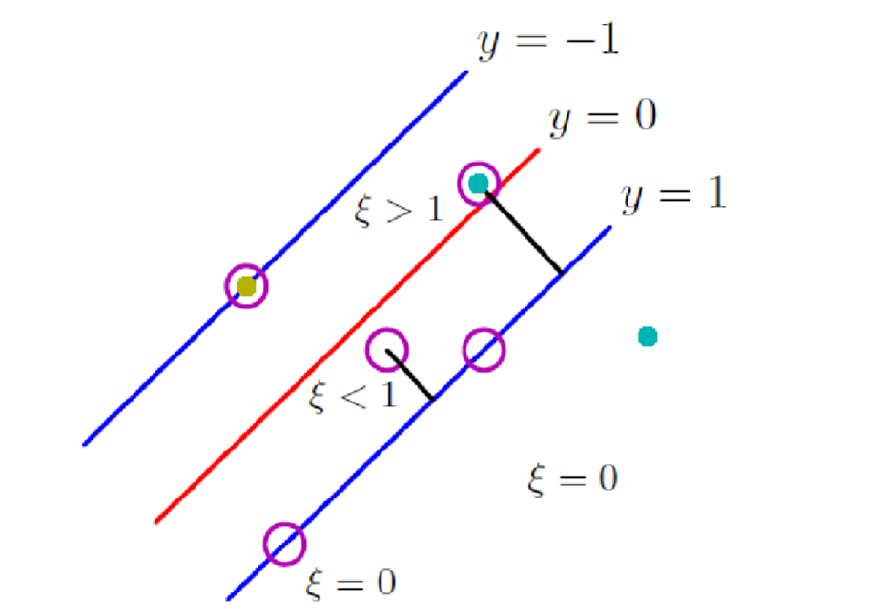
\includegraphics[height = 4cm, keepaspectratio]{graphes/ecart.png}
		\caption{[C. Bishop, Pattern Recognition and Machine Learning, Springer 2006]}
			%\end{subfigure}
	\end{center}
\end{figure}
\paragraph{}
Nous définissons les variables d'écart $\xi_i$ comme suit :
\begin{itemize}
\item[$\bullet$]  $\xi_i = 0$ si $x_i$ est bien classé	  	  	 
\item[$\bullet$]  $\xi_i = |y_i - f(x_i)|$ si $x_i$ est mal classé	  
\end{itemize}	

\paragraph{}
Le problème de maximisation de la marge devient, en introduisant la constante de régularisation $C>0$ qui pénalise d'autant plus l'erreur quelle est grande: 
\[
	\left\{
	\begin{array}{ccc}		
	\begin{aligned}
		&\text{arg}\ \text{min}_{w,b}\ \frac{1}{2}||w||^{2} + C \sum_i {\xi_i} \\
		&\forall \ 1 \leqslant i \leqslant N,\ y_i (w \cdot \phi(x_i) + b)\geqslant 1 - \xi_i \\
		&\forall \ 1 \leqslant i \leqslant N, \xi_i \geqslant 0
	\end{aligned}
\end{array}
	\right.
% − \sum{ \lambda_{i} (y_{i} (w \cdot x_i + b)−1)}
\]
Ce qui nous amène de la même manière au problème dual :
\[
\left\{
\begin{array}{lll}
	\text{max}\ L(\lambda) = \sum_{i}{\lambda_{i}} - \frac{1}{2} \sum_{i}{\sum_{j}	{\lambda_{i} \lambda_{j} y_i y_j K(x_i,x_j)}} \\
 \forall \ 1 \leqslant i \leqslant N, 0 \leqslant \lambda_i < C \\
 \forall \ 1 \leqslant i \leqslant N, \sum_{i}\lambda_i y_i = 0 
\end{array}
\right.
\]
%%%%%%%%%%%%%%%%%%% section 2 %%%%%%%%%%%%%%%%%%%%%%%%%%%%%%%%%%%%%%%%%%
\section{Application des méthode de noyaux à la Ridge Regression}
%%%%%%%%%%%%%%%%%%%%%%%%%%%%%%%%%%%%%%%%%%%%%%%%%%%%%%%%%%%%%%%%%%%%%$
La régression linéaire classique d'observations $(x_{i},\ y_{i})_{1 \leqslant i \leqslant N}$ par une fonction $f(\overset{\sim}{x}) = \langle w,\overset{\sim}{x}\rangle$ correspond au problème de minimisation :
\[
\underset{w \in \mathbb{R}^{n}}{\text{arg min}}\sum{(f(x_i) - y_i)^{2}}
\]
La regression ridge consiste à ajouter une fonction de coût avec une norme $|.|_{L^2}$ à cette erreur avec un paramètre $\lambda\geqslant 0 $ :
\[
\underset{w \in \mathbb{R}^{n}}{\text{arg min}}\sum{(f(x_i) - y_i)^{2}} +  \lambda ||w||_2^{2}
\]
\paragraph{}
L'ajout de cette pénalisation dans une régression permet par la réduction des coefficients de palier à des descripteur corrélés. Cela permet également en introduisant un biais de réduire la variance, et ainsi de réduire également l'erreur totale du modèle comme somme du biais et de la variance.
\paragraph{}
En reprenant les parties précédentes avec l'astuce du noyaux la fonction $f$ devient $f(\overset{\sim}{x}) = \sum_{i = 1}^{n}{\alpha_i \text{K}(x_i , \overset{\sim}{x})}$,et le problème de minimisation devient 
\[
\underset{\alpha \in \mathbb{R}^{n}}{\text{arg min}}\sum{(f(x_i) - y_i)^{2}} +  \lambda ||f||_H^{2}
\]
avec $H$ l'espace de Hilbert explicité dans la partie 2.2. \\
On peut ainsi écrire matriciellement ce problème :
\[
	\underset{\alpha \in \mathbb{R}^{n}}{\text{arg min}}<K \alpha - y , K 	\alpha -y > + \lambda \alpha^{T} K \alpha 
\]
$\text{où } K \in \mathbb{R}^{n \times n} \text{ est la matrice du 			noyaux} \quad K_{i,j} = K(x_i, x_j)$. \\
On trouve directement une solution analytique en prenant le gradient à 0 :
\[
\alpha	=(K + \lambda I)^{-1}y, \quad \text{avec $I$ la matrice identité}
\]
On peut donc directement exprimer les coefficients $\alpha_i$ à partir du coéfficent de pénalisation $\lambda$ et c'est ce que nous faisons dans la suite.


%%%%%%%%%%%%%%%%%%%%% chapitr 2 %%%%%%%%%%%%%%%%%%%%%%%%%%%%%%%%%%%%%%
\chapter{Experimentations}
%%%%%%%%%%%%%%%%%%%%%%%%%%%%%%%%%%%%%%%%%%%%%%%%%%%%%%%%%%%%%%%%%%%%%
\section{Évaluations des modèles}
%%%%%%%%%%%%%%%%%%%%%%%%%%%%%%%%%%%%%%%%%%%%%%%%%%%%%%%%%%%%%%%%%%%%
Nous allons dans cette partie expliciter les outils que nous allons utiliser pour évaluer les performances des modèles en comparant les prédictions $f(x_i)$ et les données $y_i$. Nous utilisons des fonctions de coût qui représentent l'erreur du modèle, on cherche à les avoir les plus petites possible. 
Nous pouvons d'abord définir la somme des résidus au carré RSS (residual sum of squares) : 
\[
\text{RSS} = \sum_{i=}^n {(y_i - f(x_i))^2}
\] 
\paragraph{}
Le premier outil est la racine de la moyenne des sommes des résidus
RMSE (root mean squared error) : 
\[
\text{RMSE} = \sqrt{\frac{1}{n}\sum_{i=}^n {(y_i - f(x_i))^2}}
\] 
Nous utilisons aussi la moyenne des erreurs absolues MAE (mean absolute error)
\[
\text{MAE} = \frac{1}{n}\sum_{i=}^n {|y_i - f(x_i)|}
\] 
L'intérêt d'utiliser deux fonctions de coût différentes et qu'elles ne donnent pas le même poids au résidus, ici l'erreur RMSE par la mise au carré va pénaliser encore plus fortement les résidus importants.

\paragraph{}
Nous utilisons également le coefficient de corrélation $R^2$
définis par 
\[ (1 - R^2) \sum_{i=1}^n {(\overline{y} - y_i)^2} \]
où $\overline{y}$ est la moyenne des observation $y$.

\paragraph{}
Nous pouvons interpréter $R^2$ comme la proportion de la variance de nos données qui sont expliqués par le modèle. Plus $R^2$ est proche de 1, plus le modèle est explicatif.






%%%%%%%%%%%%%%%%%%%%%%%%%%%%%%%%%%%%%%%%%%%%%%%%%%%%%%%%%%%%%%%%%%%%%%%%%%%
\section{noyaux pour la SVM}
\paragraph{}
Nous explicitons les différents noyaux $K$ que nous allons utiliser dans nos modélisations.\\

\paragraph{Noyaux Gaussien} 
Nous définissons le noyaux gaussien définis par :
\[ 
	K(x,z) = \exp{- \frac{||x-z||_{2}^2}{2\sigma^2}} \, \quad \sigma \geqslant 0 
\]
Ce noyaux comporte un hyperparamètre $\sigma$ à déterminer.
\begin{figure}[!h]
	\begin{center}
	%\begin{subfigure}[b]{0.3\textwidth}
		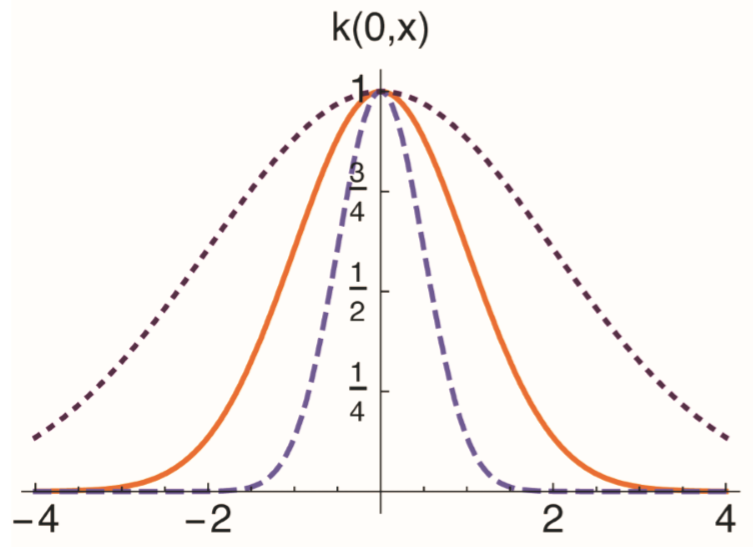
\includegraphics[height = 5cm, keepaspectratio]{graphes/noyaux_gaussien.png}
		\caption{noyaux gaussien avec $\sigma$ = 0.5 ($-$ $-$), 1 (---), 2 ($\cdot\cdot\cdot$) [Mathias Rupp \textit{Machine Learning for Quantum Mechanics in a Nutshell}]}
			%\end{subfigure}
	\end{center}
\end{figure}

\paragraph{Noyaux linéaire} Nous définissons le noyaux linéaire par :
\[ 
	K(x,z) = \langle x,z\rangle
\]
Ce noyaux ne fait pas subir de changement de dimensions, il fait comme si nous n'appliquions pas ka méthode du noyaux.

\paragraph{Noyaux Lagrangien}
Nous définissons le noyaux gaussien définis par :
\[ 
	K(x,z) = \exp{- \frac{||x-z||_{1}}{\sigma}} \, \quad \sigma \geqslant 0 
\]
Ce noyaux comporte un hyperparamètre $\sigma$ à déterminer.
\begin{figure}[!h]
	\begin{center}
	%\begin{subfigure}[b]{0.3\textwidth}
		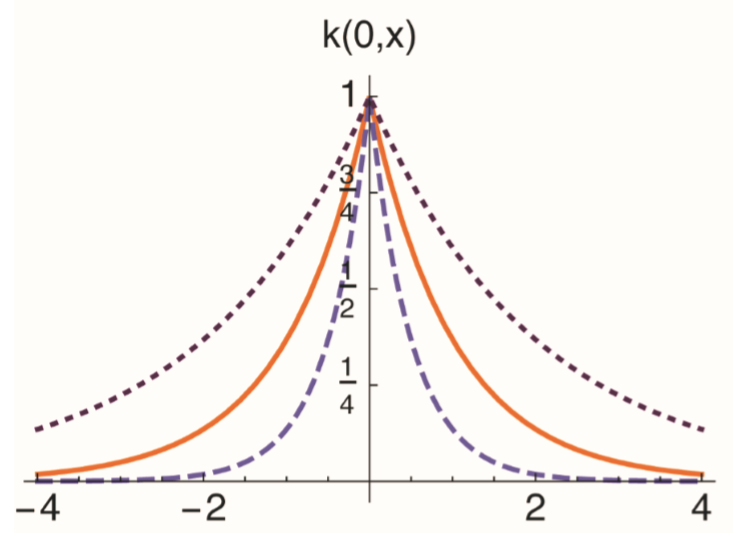
\includegraphics[height = 5cm, keepaspectratio]{graphes/noyaux_laplacien.png}
		\caption{noyaux laplacien avec $\sigma$ = 0.5 ($-$ $-$), 1 (---), 2 ($\cdot\cdot\cdot$) [Mathias Rupp \textit{Machine Learning for Quantum Mechanics in a Nutshell}]}
			%\end{subfigure}
	\end{center}
\end{figure}

\paragraph{Hyperparamètres}
Nous voyons que nous avons globalement deux hyperparmètre à determiner dans  les modèle utilisant la kernel regression ridge :
\begin{enumerate}
 	\item $\lambda$ de la ridge régression
    \item $\sigma$ du noyaux gaussien
\end{enumerate}
Nous n'utilisons pas la marge permissive avec une pénalisation ajustable décrite dans la partie 2.3.
\paragraph{}
Nous allons ainsi dans la recherche du meilleur modèle pour prédire les énergie d'atomisation des molécules nous  particulièrement à déterminer le meilleur couple d'hyperparamètres $(\lambda, \sigma)$ sur un ensemble $\Omega$ en utilisant les outils d'estimation de l'erreur d'écrits dans la section 3.1. 

%%%%%%%%%%%%%%%%%% section 2%%%%%%%%%%%%%%%%%%%%%%%%%%%%%
\section{bases d'entraînement et de test des modèles}

\paragraph{}
Nous allons détailler notre manière de procéder visant à obtenir le meilleur modèle de régression pour prédire l'énergie d'atomisation des molécules.

\paragraph{}
Tout d'abord nous allons séparer notre dataset en une base d'apprentissage sur laquelle entrainer nos modèles, et une base de test où nous évaluerons les performances des modèle avec les outils décrits section 3.1. 
\paragraph{}
Notre dataset contient un peu plus de 7000 molécules, nous le partitionnons ainsi en un training set de 1000 molécules, et un testing set contenant le reste des molécules.
\paragraph{}
Nous décomposons encore cette base d'entrainement training set de taille 1000 en une base de taille 900 pour le choix des hyperparamètres et une base de taille 100 sur laquelle nous allons vérifier la pertinence du choix de nos hyperparamètres avant de passer au modèle global, pour se prémunir contre des problème d'overfitting.
\paragraph{}
Après sélections de nos hyperparamètres, nous entrainons le modèle final sur l'ensemble du training set de 1000 molécules et nous confrontons nos prédictions aux molécules du testing set.

\paragraph{} 
Par ailleurs si nous nous intéressons à la répartition du nombre d'atome qui ne sont pas des atomes d'hydrogène par molécules dans notre dataset, nous pouvons voir sur la Figure 3.3 que cette répartition est trés inégale. En pratique nous prendrons toutes les molécules qui comprennent moins de 5 non-H atomes dans la base d'apprentissage training set car leur nombre est trés réduit (il y en a 59), même si cela augmente l'erreur de notre modèle car nos prédictions se font alors uniquement sur des molécules comportant plus de 5 atomes qui ne sont pas des atomes d'hydrogènes.
\begin{figure}[!h]
\begin{center}
		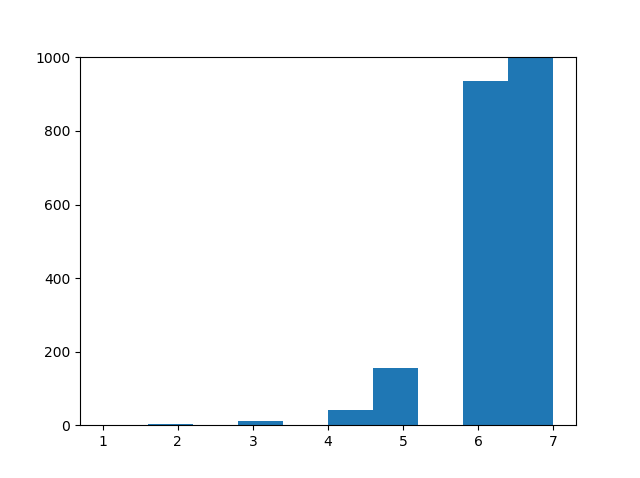
\includegraphics[height = 4.5cm, keepaspectratio]{graphes/non_H_atom.png}
		\caption{Histogramme du nombre d'atome non-H par molécule}
		\end{center}
\end{figure}

%%%%%%%%%%%%%%%%%%%%%%%%%%%%%%%%%%%%%%%%%%%%%%%%%%%%%%%%%%%%%%%%%%%%%%%%%%%
\section{Résultats}
Sur le Github \url{https://github.com/pierrzacharias/Projet_3A}, les simulations effectuées dans cette section sont réalisées dans \textit{implementation{$\_$}KKR.py} dans le fichier \textit{Methode{$\_$}Kernel{$\_$}Ridge{$\_$}Regression/}. \\
Les résultats des simulations sont stockés dans des fichiers texte tels que \\
\textit{Resultat{$\_$}RMSE{$\_$}RBF.txt} (pour l'erreur RMSE avec le noyaux gaussien), et la mise en forme des données pour l'affichage et réalisé dans  \textit{lecture{$\_$}donnee.py}.

\paragraph{Résultats pour le noyaux gaussien}
On affiche les résultats des calculs des erreurs sur une grille $(\lambda,\gamma) = [-30,-10]^2$. \\
On fait la distinction entre $\sigma$ utilisé dans l'article, et $\gamma$ utilisé dans le code avec $\gamma = \frac{1}{2\sigma^2}$

	\begin{figure}[!h]	
		\begin{center}
		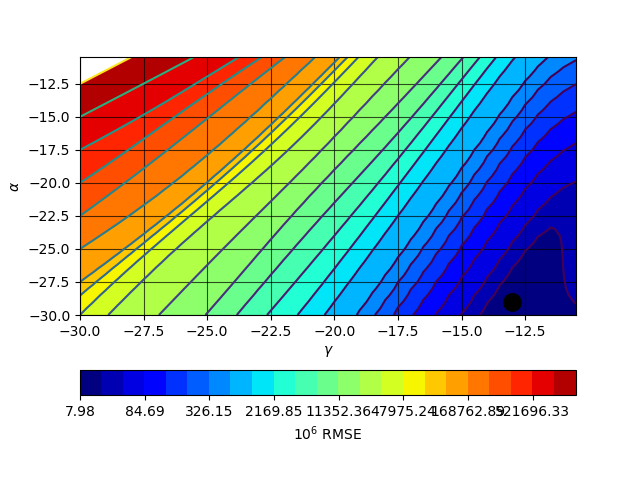
\includegraphics[height = 5cm, keepaspectratio]{graphes/resultat_RBF_RMSE.png}
		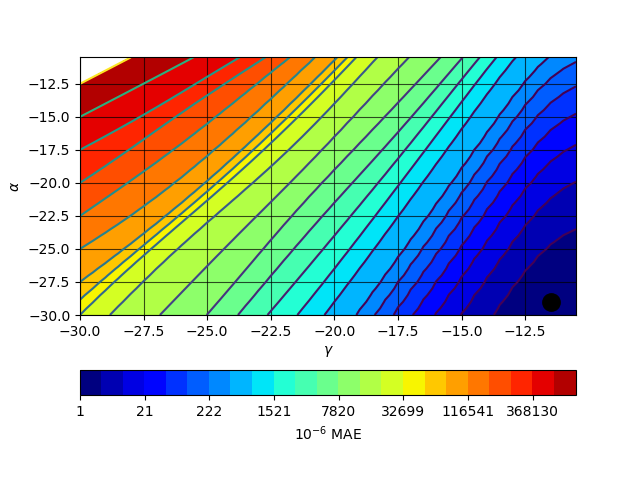
\includegraphics[height = 5cm, keepaspectratio]{graphes/resultat_RBF_MAE.png}
		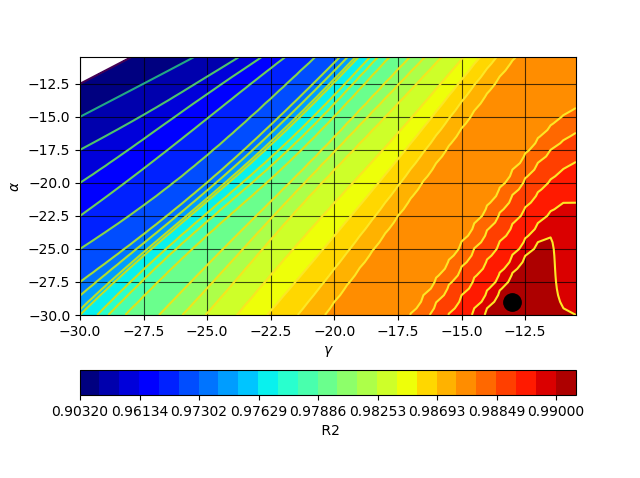
\includegraphics[height = 5cm, keepaspectratio]{graphes/resultat_RBF_R2.png}
	\caption{Résultat des modèles pour un noyau gaussien, le point noir en [-13,-29] correspond au minimum de l'erreur de l'erreur RMSE sur la grille}
		\end{center}
	\end{figure}
\paragraph{}
Nous regroupons les résultats des erreurs pour la prédiction sur le jeu de données complet : \\
\begin{center}
\begin{tabular}{ l| c c c }

   Erreur utilisée  & RMSE & MAE & R$^2$ \\
   \hline
   KRR avec noyaux gaussien & 10.3356 & 11.0503 & 0.9977\\
   KRR avec noyaux laplacien  & 10.3356 & 11.0503 & 0.9977\\
  \end{tabular}
  \end{center}
  
  
  
  
  
\end{document}
